\input{C:/Users/Christoph/OneDrive/Schule/intro.tex}
\usepackage{listings}


%\begin{lstlisting}[language=Java, lineskip={0pt}]
%\hfill{\underline\qquad /2}
\begin{document}\noindent
	\begin{tabular}{r | l}
		\includegraphics[scale = 0.1]{C:/Users/Christoph/OneDrive/Schule/HTL_IF} &
		\Huge{Übungen Klausur}\\
		\hline
	\end{tabular}\\

\section{Spring}


\subsection{Reservations}
Zu schreiben ist ein Restful Backend für eine Restaurantreservierung mit Spring. Beachten Sie die Tests.
Entwickeln Sie
\begin{itemize}
	\item Entity-Klassen kompatibel zu \texttt{data.sql}
	\begin{itemize}
		\item Guest 
		\begin{itemize}
			\item Auto-generated Primary-Key vom Typ \texttt{identity}
			\item String \texttt{name}
		\end{itemize}
		\item Table
		\begin{itemize}
			\item Auto-generated Primary-Key vom Typ \texttt{identity}
			\item Integer \texttt{size} - Anzahl Sitze
		\end{itemize}
		\item Reservation
		\begin{itemize}
			\item Auto-generated Primary-Key vom Typ \texttt{identity}
			\item ein Tisch wird reserviert (non-\texttt{null})
			\item auf einen Gast (non-\texttt{null})
			\item an einem bestimmten Datum zu einer bestimmten Uhrzeit\footnote{\texttt{LocalDateTime}, Zeitzonen sind zu ignorieren} in der Zukunft
			\item für eine positive Anzahl Personen
		\end{itemize}
	\end{itemize}
	\item Rest-Endpoints
	\begin{itemize}
		\item \texttt{get /reservations?name=guestName}\\
		Liefert eine \texttt{List} aller Reservierungen auf Gäste mit Namen \texttt{guestName}
		\item \texttt{get /reservations/{id}}\\
		Liefert die Reservierung mit der übergebenen \texttt{id} oder \texttt{NOT\_FOUND}
		\item \texttt{post /reservations}\\
		Speichert eine neue Reservierung. Dabei ist zu beachten:
		\begin{itemize}
			\item Status \texttt{CREATED} bzw \texttt{BAD\_REQUEST}
			\item Location im Response-Header ist gesetzt
			\item Die Personenanzahl, für die reserviert wird muss kleiner gleich der \texttt{Table.size} sein.
			\item Eine Reservierung blockiert einen Tisch für 2 Stunden(exklusive der letzten Sekunde), also wenn eine Reservierung für X existiert, kann keine Reservierung mit Beginnzeitpunkt (X-2):00:01 - (X+1):59:59 gespeichert werden.
		\end{itemize}
	\end{itemize}
	\item einen zentralen Exception-Handler
\end{itemize}

\subsection{Space-history}
Zu schreiben ist eine MVC-Webapplication mit Spring und Thymeleaf.

Im module \texttt{space-history} finden Sie einige Rohklassen. Der gegebene Code kann beliebig modifiziert werden, es ist nur \textbf{nicht} empfohlen, den \texttt{DateTimeFormatter} in \texttt{CsvParser} zu ändern.
Entwickeln Sie 
\begin{itemize}
	\item eine Entitätsklasse \texttt{Launch}, \texttt{id} beliebig
	\item eine Implementierung von \texttt{CsvParser}, welche die gegebene Datei \texttt{space-history.csv} in entsprechende \texttt{Launch}-Objekte parst.\footnote{Temporär bzw. falls Sie bei diesem Punkt scheitern können sie mit den Daten aus \texttt{getStartingData} arbeiten.}
	\begin{itemize}
		\item \texttt{Location} wird nicht verwendet
		\item \texttt{Date} kann durch den gegebenen \texttt{DateTimeFormatter} gelesen werden
		\item \texttt{Detail} enthält bis zum ersten \texttt{|} den Namen der Rakete, danach folgen Details über die Mission. 
		\item \texttt{Status Rocket} wird nicht verwendet
		\item \texttt{Rocket} enthält nicht den Namen der Rakete sondern meist gar nichts oder die Schubkraft
		\item \texttt{Status Mission} enthält Daten über den Erfolg der Mission. Zu unterscheiden ist einzig zwischen \texttt{Success} und \texttt{Failure}\footnote{Die Art des Scheiterns ist irrelevant}.
		\item Sie können die Datei auch parallel zur \texttt{pom.xml} ablegen, allerdings wirkt sich dies negativ auf die Beurteilung aus.
	\end{itemize}
	\item folgende Webseiten:
	\begin{itemize}
		\item Eine Übersicht aller Launches
		\begin{itemize}
			\item \textbf{absteigend} sortiert nach Datum.
			\item Der Name der Company ist ein Link zu einer ähnlichen Seite, bei der nur Missionen dieser Company aufscheinen.
			\item Mittels eines Links gelangt man zu einer Seite für das Registrieren einer neuen Mission.
		\end{itemize}
		\fbox{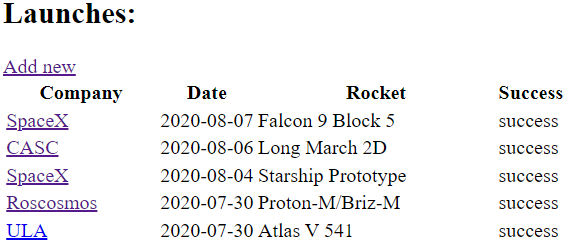
\includegraphics{all-launches}}
		\item Eine Übersicht aller Launches \textbf{einer} Company \textbf{absteigend} sortiert nach Datum.\textbf{}
		\fbox{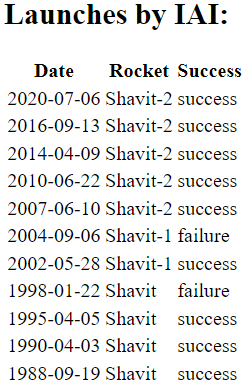
\includegraphics{launches-iai}}
		\item Ein Formular zum Erfassen eines neuen Launches
		\begin{itemize}
			\item Company: Dropdown-Selection für alle bekannten Companies
			\item Date: Datepicker (nicht null, maximal heute), Format beliebig
			\item Rocket: Freitext, kann null sein
			\item Success: Checkbox
			\item Im Erfolgsfall redirect zur Übersicht aller Launches
			\item Im Fehlerfall ist eine entsprechende Fehlermeldung anzuzeigen und die Eingabeseite mit den fehlerhaften Daten neu zu laden
		\end{itemize}
		\fbox{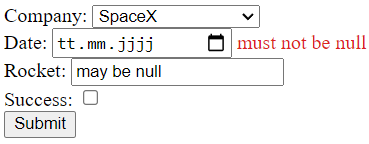
\includegraphics{new-launch-date-null}} \\
		\fbox{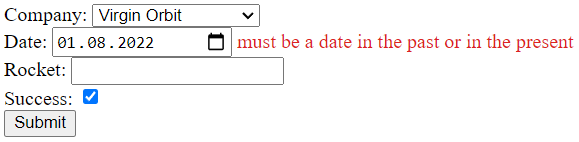
\includegraphics{new-launch-date-future}}
	\end{itemize}
\end{itemize}

\subsection{Geography}
Entwickeln Sie
\begin{itemize}
	\item Entity-Klassen kompatibel zu \texttt{data.sql}
	\begin{itemize}
		\item City 
		\begin{itemize}
			\item Auto-generated Primary-Key vom Typ \texttt{identity} 
		\end{itemize}
		\item Country
		\begin{itemize}
			\item Primary-Key \texttt{code} ist exakt 2 Character lang
			\item \texttt{name} beginnt mit einem Großbuchstaben
		\end{itemize}
	\end{itemize}
	\item Rest-Endpoints
	\begin{itemize}
		\item \texttt{get /countries/\{code\}}\\
		Liefert das Country mit \texttt{code} oder \texttt{NOT\_FOUND}
		\item \texttt{post /countries}\\
		Speichert eine neues Country. Dabei ist zu beachten
		\begin{itemize}
			\item Status \texttt{CREATED} bzw \texttt{BAD\_REQUEST}
			\item Location im Response-Header ist gesetzt
			\item Es darf noch kein Country mit diesem \texttt{code} existieren
		\end{itemize}
	\end{itemize}
	\item einen zentralen Exception-Handler
	\item folgende Webseiten:
	\begin{itemize}
		\item Eine Übersicht aller Countries mit den entsprechenden Cities darunter
		\begin{itemize}
			\item show cities ändert den unteren Teil der Seite
		\end{itemize}
		\fbox{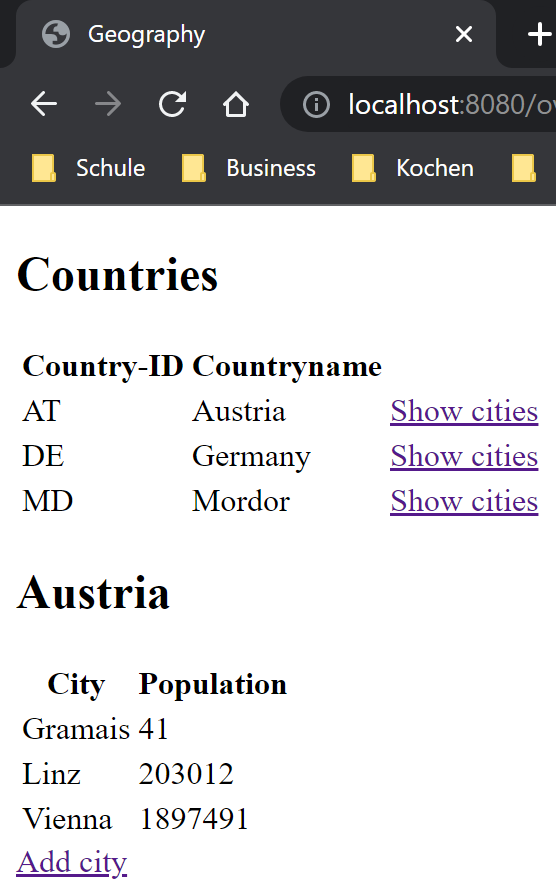
\includegraphics[scale=1]{austria-cities}}
		\item Ein Formular zum Erfassen einer neuen City\\
		\fbox{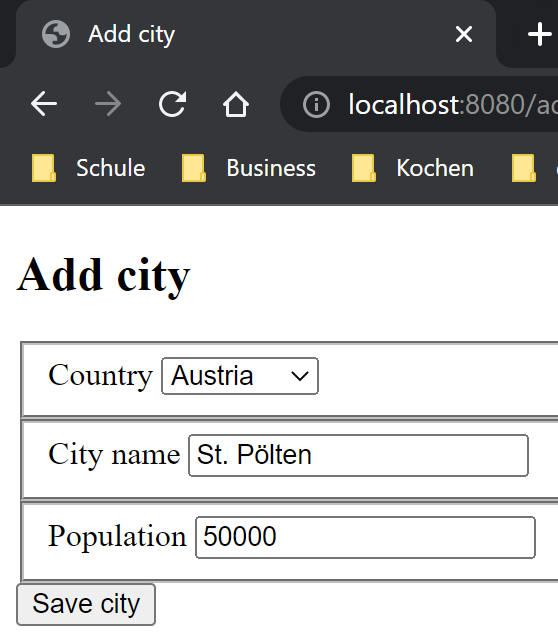
\includegraphics{add-city}}\\
		\begin{itemize}
			\item Im Erfolgsfall redirect zur Übersicht des jeweiligen Landes
			\item Im Fehlerfall ist eine entsprechende Fehlermeldung anzuzeigen und die Eingabeseite mit den fehlerhaften Daten neu zu laden
		\end{itemize}
	\end{itemize}
\end{itemize}

\section{Tests}
Schreibe Tests zu den Methoden der Klasse \texttt{Service} in \texttt{testing}.

\section{Logik}
\subsection{Checkout}
Zu schreiben ist Software für eine Supermarktkasse.

\begin{itemize}
	\item \texttt{Price} - Preis eines Artikels
	\item \texttt{Item} - ein konkreter Artikel, welcher eingekauft wird, \textbf{ein} Apfel \\
	\texttt{equals}/\texttt{hashCode} ist derartig implementiert, dass es nur auf das \texttt{Produkt} ankommt, das zum Artikel gehört
	\item \texttt{Product} - Artikel, welche verkauft werden, \textbf{alle} Äpfel \\
	\texttt{equals}/\texttt{hashCode} ist derartig implementiert, dass es nur auf die \texttt{description} des Produkts ankommt, es gibt also nur \textbf{eine} Art von Äpfeln
	\item \texttt{Offer} - Angebot, x Stück eines Artikels um einen bestimmten Preis
\end{itemize}

\begin{enumerate}
	\item Schreiben Sie in \texttt{CheckoutTest} einen UnitTest für die Methode \texttt{filter}.
	\item Schreiben Sie nötigen Code, sodass alle Tests passen.
\end{enumerate}

\subsection{Orbits}
In einer Simulation umkreisen Himmelskörper einander. Dies wird durch einen Graphen modelliert. 
\begin{itemize}
	\item Der Graph wird durch Strings beschrieben, wobei \texttt{a)b} bedeuten soll, dass \texttt{b} um \texttt{a} kreist.
	\item Der Root-Knoten sei jener, der selbst um nichts kreist.
	\item Wenn wir annehmen, dass alle Himmelskörper gleich weit voneinander weg sind, liefert \texttt{totalDistance} die Gesamtdistanz zum Root.
\end{itemize}

\subsection{Build-Planner}
Ein Projekt besteht aus mehreren Schritten, wobei viele Schritte andere voraussetzen. Der Input kommt in Form von Strings ähnlich
\begin{verbatim}
	"Step B must be finished before step A can begin."
	"Step C must be finished before step A can begin."
\end{verbatim}

\begin{itemize}
	\item Die Klasse \texttt{BuildPlanner} bekommt derartige Strings übergeben und verarbeitet sie
	\item \texttt{getRequirementsForStep} retourniert eine \texttt{SortedMap}, welche als key die Schritte speichert und als value ein \texttt{Set} jener Schritte, die für den jeweiligen key Voraussetzung sind
	\item \texttt{order} erzeugt eine \texttt{Queue} der Schritte in der richtigen Reihenfolge
	\item Ungültige Strings werden ignoriert, Zyklen oder anderer unsinniger Input resultiert in einer \texttt{order}-Exception
\end{itemize}

\section{Design Pattern}
\subsection{Censorship}
Zu schreiben ist Code, um eine Zensur umzusetzen.

\begin{itemize}
	\item Sie haben eine Applikation zum Parsen von JSON geschrieben, welche vortrefflich funktioniert, allerdings möchte ihr neuester Kunde ein neues Feature. 
	\item Der Kunde wünscht, dass falls der JSON-String \textbf{irgendwo caseinsensitive} ein Wort aus der \texttt{forbidden.txt} enthält, das Parsing abgebrochen wird und eine \texttt{RuntimeException} geworfen wird. \\
	\begin{verbatim}
		{
			"title": "Analysis of african soils",
			"author": "Angie smith"
		}
	\end{verbatim}
	enthält beispielsweise die verbotenen Worte "anal", "africa", "african" und "angie". \\
	Ein einzelnes dieser Worte im übergebenen JSON reicht, dass der gesamte JSON zu verwerfen ist. 
	\item Weil Sie mit dem Open Closed Principle vertraut sind und da die Applikation komplett ungetestet ist, entscheiden Sie sich dagegen, im vorhandenen Code Änderungen vorzunehmen, sondern ein Design Pattern zur Lösung einzusetzen.
	\item \textbf{Die Methode \texttt{decode} in \texttt{Decoder} darf nicht verändert werden}, alles andere schon. 
\end{itemize}

\begin{enumerate}
	\item Generieren/Zeichnen Sie ein problemangepasstes UML-Diagramm, das die Struktur des Patterns zeigt.
	\item Führen Sie die notwendigen Änderungen im Code durch. 
	\item Sie müssen keine Tests schreiben, sondern können mit Hilfe der \texttt{main}-Methode testen. 
\end{enumerate}

\subsection{Circle-shape}
Sie müssen eine awt-Application in eine JavaFX-Application portieren. Dazu muss \texttt{Circle} \texttt{Shape} implementieren. Ein Klasse \texttt{Circular} ist bereits in der Applikation vorhanden und soll weiterverwendet werden.
\begin{itemize}
	\item Generieren/Zeichnen Sie ein problemangepasstes UML-Diagramm, das die Struktur des Patterns zeigt.
	\item Führen Sie die notwendigen Änderungen im Code durch. 
\end{itemize}

\subsection{Output}
\begin{itemize}
	\item Welches Designpattern wurde implementiert?
	\item Welche Rollen spielen die Klassen OutputChannel und OutputFilter im Pattern?
	\item Geben Sie einen use-case für das Pattern an
\end{itemize}

\subsection{Coffee}
	Sie sollen Software für eine Kaffeehauskette schreiben, welche verschiedenste Möglichkeiten für Kaffee anbietet:
	\begin{itemize}
		\item nur Kaffee
		\item Kaffee mit Milch(Hafer? Soja? Kuh?)
		\item Kaffee mit Sirup(Karamel? Vanille?)
		\item Kaffee mit Zucker
	\end{itemize}
\begin{itemize}
	\item Erstellen Sie Klassen, welche beliebige Kombinationen ermöglichen. Für jedes derartige Produkt soll ein Gesamtpreis und eine Liste der Zutaten abgerufen werden können.
	\item Schreiben Sie einige Tests für ihre Application. 
\end{itemize}

\end{document}